In order to test our theory we implemented a tool-chain for
the identification of weaknesses and the precise calculation of 
potential insecure configurations. In this section, we describe
the tool-chain and the concepts related to the risk estimantion, 
such as likelihood and impact of attack paths.

The engineering of the $\abftheory$ is summarized in the UML Class
diagram in Figure~\ref{fig:secraclassdiagram}. The Class diagram
represents the concepts introduced in Section~\ref{sec:engineering}.
\begin{sidewaysfigure}
	\centering
	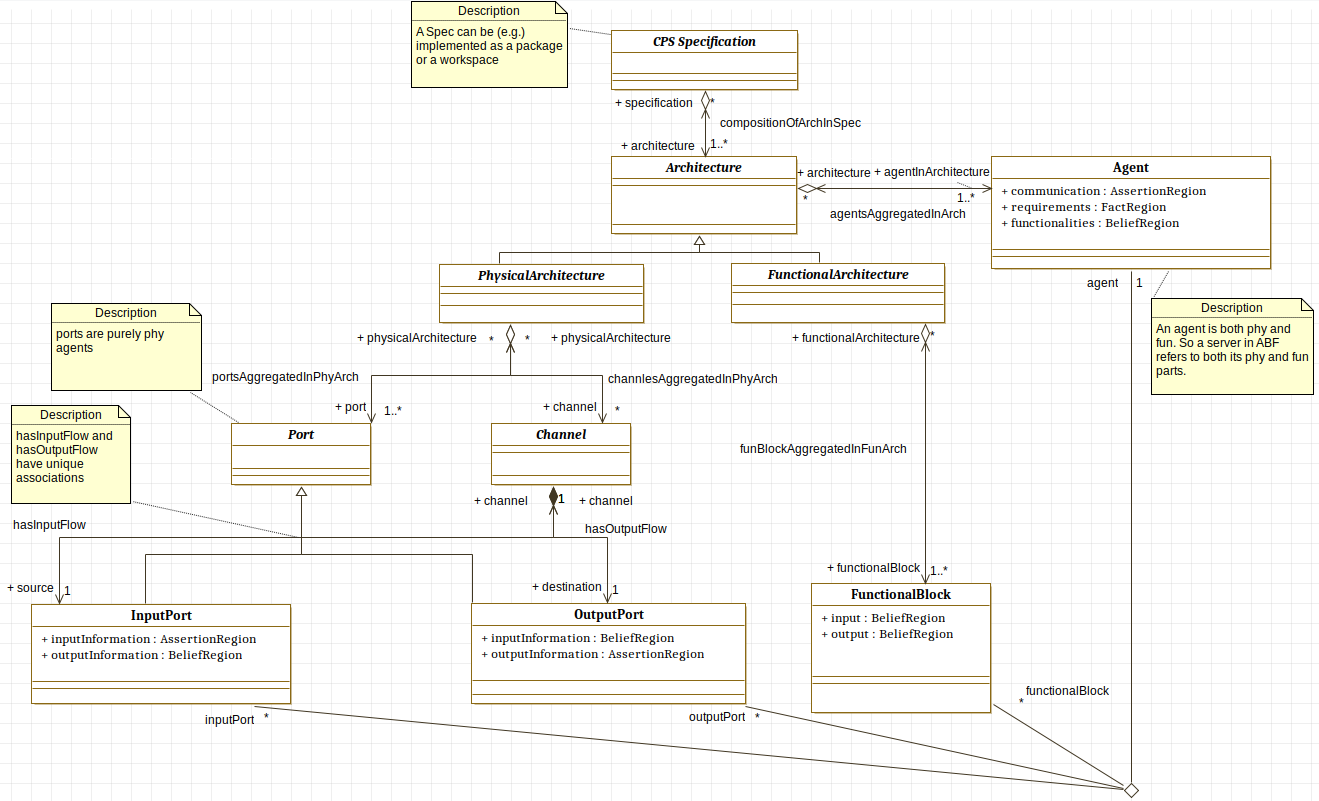
\includegraphics[width=\textwidth]{secra_classDiagram.png}
	\caption{Security Risk Assessment -- Class Diagram}
	\label{fig:secraclassdiagram}
\end{sidewaysfigure}
This allows us to define a CPS as a composition of the two (symmetric)
structures depicted in Figure~\ref{fig:molecules}. A system can be
designed in $\abftheory$ as the composition of structures formed
by 3 elements: functional architecture, ports, and channels.
If the information flows from left to right the port is an output port,
otherwise (right-to-left) is an input port.
\begin{figure}
	\centering
	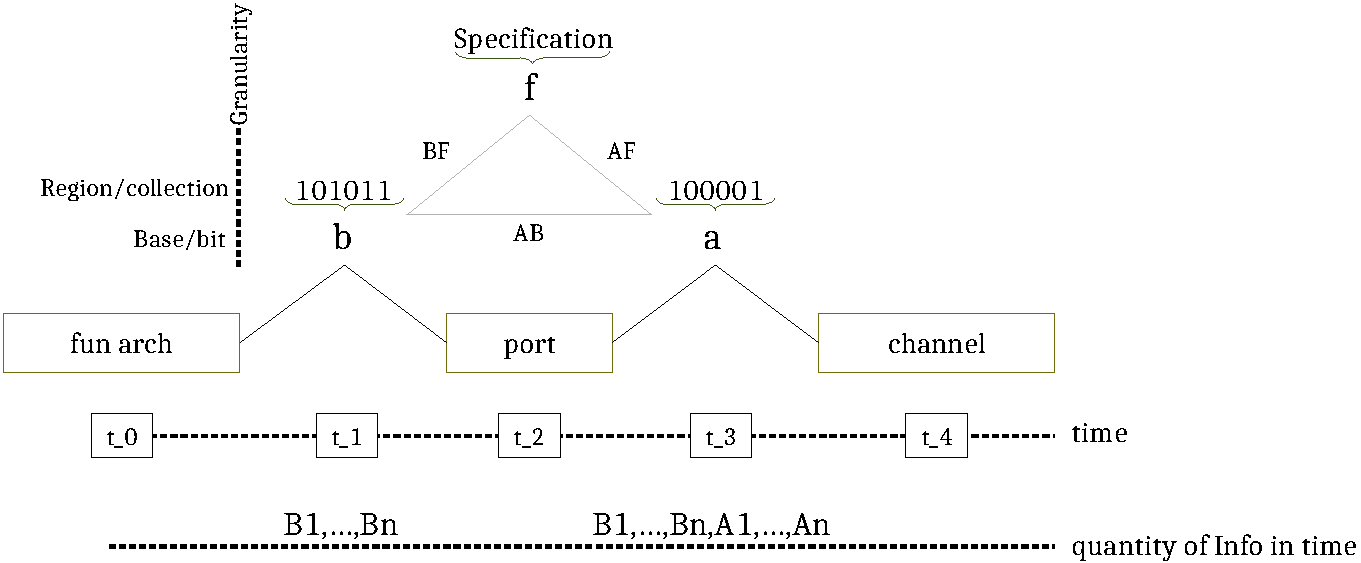
\includegraphics[width=\textwidth]{molecule.pdf}
	\caption{Summary of $\abf$ Engineering Model}
	\label{fig:molecules}
\end{figure}

\subsection{V-SecRA Tool-chain}
\begin{figure}
	\centering
	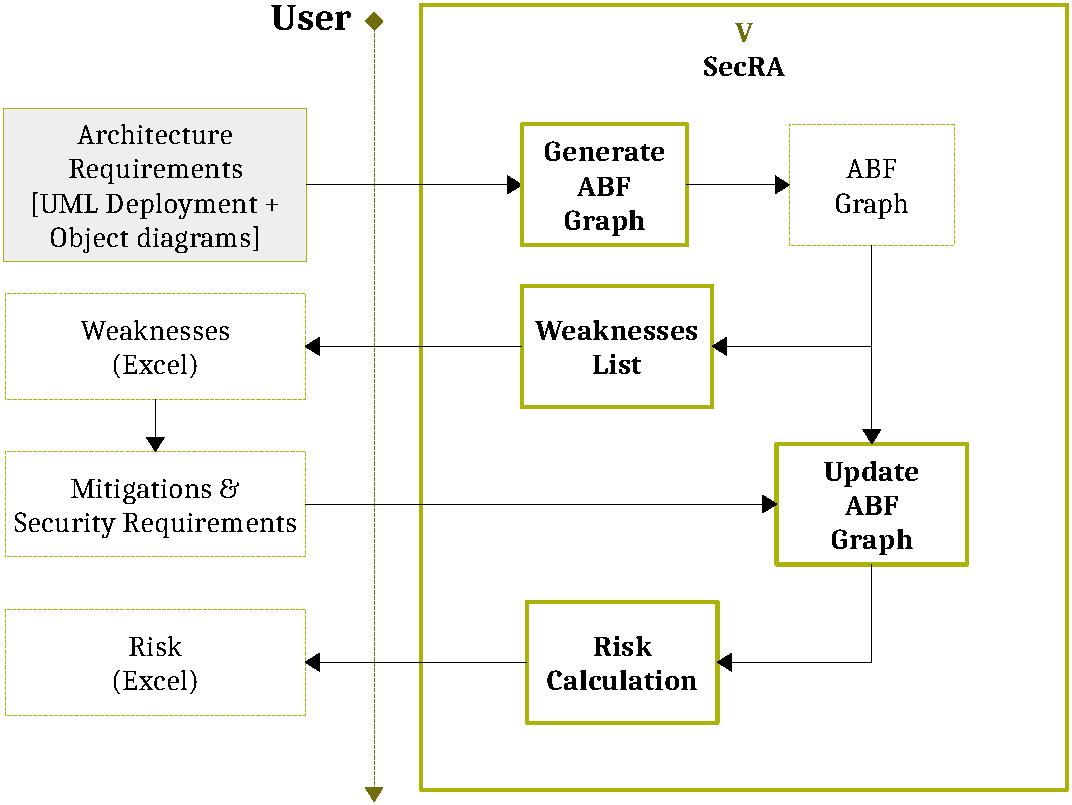
\includegraphics[width=\textwidth]{v-secra.pdf}
	\caption{V-SecRA}
	\label{fig:v-secra}
\end{figure}
The security risk assessment process starts with the definition
of the use cases (see Figure~\ref{fig:usecase}) and architectural requirements 
(see Appendix~\ref{app:requirements}); which we call specification.
In our process, the specification is translated into a UML design where:
\begin{itemize}
	\item a \emph{Deployment Diagram} describes the \emph{Physical
		Architecture}. Each agent is defined as a Node with (physical)
		Ports, and Agent's ports are connected via Information Flow
		connectors, representing the physical channel.
	\item a \emph{Functional Architecture} is linked to each agent in the
		deployment diagram and is defined by an \emph{Object Diagram}.
		The Object Diagram is composed by Instances of Functional
		Blocks, connected via Information Flow connectors.
	\item the connection between the two diagrams is implemented by
		``sockets'', functional blocks with the same name of the
		corresponding physical port.
\end{itemize}

\subsection{Impact and Likelihood}\label{sec:impact}
As described in~\autocite{CORASMethod}, in order to quantitatively estimate the
cybersecurity \emph{risk} of a CPS design, one needs to estimate both the
\emph{likelihood} of \emph{attack paths} (attack from now on)\fixnote{mr}{check terminology
consistency} along with their (negative) \emph{impact} on a requirement which, in
turn, is related to some \emph{company assets}. An attack that has a negative impact
on a requirement invalidates the requirement, leading to one or more \emph{incidents}.
